% ============================================================
%  HBCC: Kiến Trúc Lai Cục Bộ--Phân Cụm Tăng Cường Bằng
%  Chưng Cất Tri Thức Cho Phân Loại Ảnh Nhẹ
%  Phiên bản hoàn chỉnh — gộp main.tex và HBCC_paper_vi.tex
% ============================================================
\documentclass[journal]{IEEEtran}

% --- Encoding -----------------------------------------------
\usepackage[utf8]{inputenc}
\usepackage[T5]{fontenc}

% --- hyperref first (avoids IEEEtran \egroup conflict) -------
\usepackage[colorlinks=true,linkcolor=blue,citecolor=blue,urlcolor=blue,
            pdftitle={HBCC},pdfauthor={Nguyen Viet Hung},
            bookmarks=false]{hyperref}

% --- Math ---------------------------------------------------
\usepackage{amsmath}
\usepackage{amssymb}
\usepackage{bm}

% --- Figures & tables ---------------------------------------
\usepackage{graphicx}
\graphicspath{{images/}}
\usepackage{booktabs}
\usepackage{multirow}
\usepackage{array}
\usepackage{float}

% --- Misc ---------------------------------------------------
\usepackage{url}
\usepackage{cite}

% ============================================================
\begin{document}

% \texorpdfstring: TeX thấy tiêu đề UTF-8; metadata PDF dùng ASCII
\title{HBCC: Kiến Trúc Lai Cục Bộ--Phân Cụm Ngữ Cảnh
  Tăng Cường Bằng Chưng Cất Tri Thức Cho Phân Loại Ảnh}

\author{Nguyễn~Việt~Hùng,~Nguyễn~Bá~Nam,~và~Lê~Hoàng~Thái%
  \thanks{Nguyễn Việt Hùng và Nguyễn Bá Nam là
          sinh viên thực hiện nghiên cứu.
          Lê Hoàng Thái (PGS.TS.) là giảng viên hướng dẫn.
          Nhóm tác giả thuộc Trường Đại học
          Khoa học Tự nhiên, ĐHQG-HCM.
          Tác giả liên hệ: Nguyễn Việt Hùng
          (\texttt{hbinzv0108@gmail.com}).}}

\markboth{Truong DHKHTN -- DHQG HCM}%
         {Nguyen V.H. \texorpdfstring{\textit{et al.}}{et al.}: HBCC}

\maketitle

% ============================================================
\begin{abstract}
Phân loại ảnh hiệu quả trên thiết bị nhúng đặt ra bài toán đánh đổi
khó giải quyết: các kiến trúc CNN nhẹ như MobileNetV2 và ShuffleNetV2
giảm chi phí tính toán nhưng đánh đổi bằng độ chính xác thấp hơn
đáng kể, trong khi Context Cluster (CoC) dùng phân cụm ngữ cảnh thay
convolution nhưng bỏ qua kết cấu cục bộ -- yếu tố quan trọng ở độ
phân giải cao. Hơn nữa, khi áp dụng CoC trực tiếp cho ảnh nhỏ
($32\!\times\!32$), vấn đề \textit{suy biến token} xuất hiện: bước
trượt stem quá lớn khiến mỗi cụm chỉ chứa đúng một điểm và toán tử
phân cụm trở nên vô hiệu.

Bài báo này đề xuất \textbf{HBCC} (\textit{Hybrid Binarized Context
Cluster}), kiến trúc lai bốn tầng với hai câu hỏi nghiên cứu:
\textbf{(CQ1)} liệu kết hợp xử lý cục bộ và phân cụm có cải thiện
đồng thời độ chính xác và hiệu quả không? \textbf{(CQ2)} chiến lược
phân bổ nhánh cục bộ theo tầng nào là tối ưu cho ảnh $32\!\times\!32$?
Tầng 1 ($32\!\times\!32$) dùng LBPConv -- bộ lọc cố định gần như
không tốn MACs; Tầng 2 ($16\!\times\!16$) dùng DWConv với chi phí
$1/C$ so với convolution chuẩn; Tầng 3--4 ($8\!\times\!8$,
$4\!\times\!4$) dùng phân cụm thuần. Fold partitioning chia feature
map thành tile cục bộ trước phân cụm, ngăn global over-smoothing.
Chúng tôi xác định và khắc phục suy biến token bằng cách giảm bước
trượt stem từ 2 xuống 1, kết hợp thu hẹp độ sâu từng tầng. Ngoài ra,
chưng cất tri thức (KD) từ giáo viên ResNet-18 ($\alpha{=}0{,}5$,
$T{=}4{,}0$) được áp dụng như kỹ thuật tăng cường độ chính xác.

Trên CIFAR-10, HBCC-Medium+KD đạt \textbf{95,36\%} top-1 với 1,76M
tham số và 138,8M MACs, vượt ShuffleNetV2 ($+$3,68\%) và MobileNetV2
($+$4,32\%). Trên CIFAR-100, HBCC-Medium+KD đạt \textbf{77,68\%}
top-1, vượt toàn bộ các mô hình nhẹ đối chứng. HBCC-Small+KD
(1,27M tham số) vượt ShuffleNetV2 (1,26M tham số) tới $+$3,25\%
trên CIFAR-10 và $+$0,29\% trên CIFAR-100 ở cùng ngân sách tham số.
Phân tích hồ sơ toán tử giải thích vì sao tiết kiệm tham số/MACs
chưa chuyển hóa thành tiết kiệm độ trễ thực đo -- một hạn chế được
nêu rõ và đề xuất hướng giải quyết.
\end{abstract}

\begin{IEEEkeywords}
phân loại ảnh, Context Cluster, kiến trúc lai cục bộ--phân cụm,
mạng nơ-ron nhẹ, chưng cất tri thức, suy biến token, CIFAR-10,
CIFAR-100.
\end{IEEEkeywords}

% ============================================================
\section{Giới Thiệu}
\label{sec:intro}

\IEEEPARstart{P}{hân} loại ảnh là bài toán nền tảng trong thị giác máy
tính, đạt được nhiều tiến bộ nhờ mạng nơ-ron tích chập sâu
(CNN)~\cite{He2016ResNet} và Vision Transformer~\cite{Dosovitskiy2021ViT}.
Tuy nhiên, việc triển khai trên thiết bị biên (\textit{edge device})
đặt ra thách thức: ResNet-18 cần 11,17M tham số và 556,7M MACs chỉ để
xử lý ảnh $32\!\times\!32$, vượt quá giới hạn của nhiều nền tảng nhúng.

Các kiến trúc nhẹ như MobileNetV2~\cite{Sandler2018MobileNetV2} và
ShuffleNetV2~\cite{Ma2018ShuffleNetV2} giảm chi phí qua depthwise
convolution và channel shuffle, nhưng đạt độ chính xác thấp hơn đáng
kể (91,04\% và 91,68\% trên CIFAR-10, 73,75\% và 76,46\% trên
CIFAR-100 trong thực nghiệm của chúng tôi). Context Cluster
(CoC)~\cite{Ma2023ImageAsSetOfPoints} coi ảnh như tập hợp điểm 5D
$(R,G,B,x,y)$ và dùng phân cụm với chi phí $O(N\!\cdot\!M\!\cdot\!D)$,
nhưng pure clustering bỏ qua kết cấu cục bộ, dẫn đến chỉ 88,34\%
trên CIFAR-10.

Chúng tôi xác định thêm một vấn đề cấu trúc của CoC trên ảnh nhỏ:
\emph{suy biến token}. Khi bước trượt stem quá lớn, bản đồ đặc trưng
ở tầng cuối chỉ còn rất ít điểm -- bằng hoặc nhỏ hơn số tâm cụm đề
xuất -- khiến mỗi cụm chứa đúng một điểm và toán tử phân cụm trở
nên đồng nhất. Với stem\_stride=2 trên ảnh $32\!\times\!32$, Tầng~4
chỉ còn $2\!\times\!2=4$ điểm nhưng đề xuất 4 tâm, tỉ lệ điểm/cụm
bằng 1.

Bài báo này đề xuất \textbf{HBCC} (\textit{Hybrid Binarized Context
Cluster}) với các đóng góp chính:
\begin{enumerate}
  \item \textbf{Hybrid Cluster Block}: chia channel thành nhánh
        cluster (ngữ cảnh toàn cục) và nhánh cục bộ (LBPConv hoặc
        DWConv), fuse qua channel shuffle và $1\!\times\!1$ convolution.
  \item \textbf{Khắc phục suy biến token}: giảm stem\_stride từ 2
        xuống 1, kết hợp thu hẹp số khối mỗi tầng, đảm bảo mỗi cụm
        luôn có ít nhất 4 điểm thành viên.
  \item \textbf{Thiết kế tầng lũy tiến}: Tầng~1--2 dùng hybrid tại
        resolution cao nơi kết cấu cục bộ quan trọng; Tầng~3--4 dùng
        pure cluster tại $8\!\times\!8$, $4\!\times\!4$.
  \item \textbf{Chưng cất tri thức (KD)}: ResNet-18 làm giáo viên,
        được đánh giá trên cả CIFAR-10 và CIFAR-100, cho thấy KD
        đặc biệt hiệu quả trên tập khó hơn (CIFAR-100: $+$2,09\%).
\end{enumerate}

Bài báo đặt ra hai câu hỏi nghiên cứu:

\noindent\textbf{(CQ1)} Liệu kiến trúc lai kết hợp xử lý cục bộ và
phân cụm ngữ cảnh có thể cải thiện đồng thời độ chính xác và hiệu
quả tính toán so với cả thuần túy CNN nhẹ lẫn thuần túy phân cụm không?

\noindent\textbf{(CQ2)} Chiến lược phân bổ nhánh cục bộ theo tầng nào
là tối ưu cho ảnh nhỏ $32\!\times\!32$?

\noindent\textit{Phạm vi:} CIFAR-10 và CIFAR-100, ràng buộc dưới 2M
tham số. \textit{Bố cục:} Phần~\ref{sec:related} tổng quan tài liệu;
Phần~\ref{sec:arch} mô tả kiến trúc đề xuất;
Phần~\ref{sec:exp} trình bày thiết lập thực nghiệm;
Phần~\ref{sec:results} trình bày kết quả và thảo luận;
Phần~\ref{sec:limitations}--\ref{sec:conclusion} là hạn chế và kết luận.

% ============================================================
\section{Tổng Quan Tài Liệu và Cơ Sở Lý Thuyết}
\label{sec:related}

\subsection{Mạng CNN và residual learning}

ResNet~\cite{He2016ResNet} giới thiệu residual connection:
$\mathbf{y} = \mathcal{F}(\mathbf{x}) + \mathbf{x}$,
cho phép gradient truyền thẳng qua lớp, ngăn vanishing gradient và
mở ra kỷ nguyên huấn luyện mạng 50--152 lớp. Standard $3\!\times\!3$
convolution với $C_{\mathrm{in}}$ kênh vào, $C_{\mathrm{out}}$ kênh ra,
kernel size $k$ có chi phí tỷ lệ với
$C_{\mathrm{in}}\!\cdot\!k^2\!\cdot\!C_{\mathrm{out}}$, làm ResNet-18
cần 556,7M MACs dù ảnh chỉ $32\!\times\!32$.

MobileNetV2~\cite{Sandler2018MobileNetV2} thay standard conv bằng
depthwise separable conv: tách thành depthwise ($k\!\times\!k$ riêng
cho từng channel, chi phí $C_{\mathrm{in}}\!\cdot\!k^2$) và pointwise
($1\!\times\!1$, chi phí $C_{\mathrm{in}}\!\cdot\!C_{\mathrm{out}}$),
giảm tổng chi phí về $O(C_{\mathrm{in}}(k^2 + C_{\mathrm{out}}))$ --
tiết kiệm xấp xỉ $1/k^2$ lần. ShuffleNetV2~\cite{Ma2018ShuffleNetV2}
chỉ ra rằng FLOPs không tương quan trực tiếp với tốc độ thực đo và
đề xuất bốn nguyên tắc: (i) cân bằng số channel đầu vào/ra; (ii)
tránh group convolution; (iii) tránh phân nhánh kiến trúc; (iv) giảm
element-wise operations. HBCC kế thừa tinh thần này khi nhận ra rằng
các toán tử phân cụm nhỏ, phân mảnh cũng gây ra vấn đề tương tự về
độ trễ thực đo.

\subsection{Vision Transformer và MetaFormer}

ViT~\cite{Dosovitskiy2021ViT} chia ảnh thành $n$ patch và áp dụng
multi-head self-attention:
\begin{equation}
  \operatorname{Attn}(Q,K,V) =
  \operatorname{softmax}\!\!\left(\frac{QK^\top}{\sqrt{d_k}}\right)\!V,
  \label{eq:attn}
\end{equation}
với độ phức tạp $O(n^2 d_k)$. Trên ảnh $32\!\times\!32$ với patch
$2\!\times\!2$, $n{=}256$ token; chi phí $O(256^2)$ là quá lớn cho
bài toán lightweight. HBCC thay self-attention bằng phân cụm
$O(n\!\cdot\!K)$ với $K{=}4$, giảm chi phí $\approx\!64\!\times$
so với single-head attention. Các kiến trúc MetaFormer cho thấy cấu
trúc hai khối (trộn token + MLP) của Transformer quan trọng không
kém toán tử cụ thể; HBCC cũng theo mô-típ này với layer-scale.

\subsection{Context Cluster}

CoC~\cite{Ma2023ImageAsSetOfPoints} biểu diễn ảnh như tập hợp điểm
5D $(R,G,B,x,y)$, tích hợp tọa độ không gian vào đặc trưng. Cluster
centers được tạo tự động qua AdaptiveAvgPool (không tham số học);
điểm được gán cứng vào cluster gần nhất qua cosine similarity với
chi phí $O(N\!\cdot\!M\!\cdot\!D)$. Hạn chế chính: pure clustering ở
mọi tầng bỏ qua thông tin tần số cao (kết cấu vi mô, cạnh), làm
CoC-baseline chỉ đạt 88,34\% trên CIFAR-10. Ngoài ra, suy biến
token xảy ra khi bản đồ đặc trưng quá nhỏ so với số tâm cụm (phân
tích chi tiết ở Mục~\ref{sec:degeneracy}).

\subsection{Local Binary Pattern}

LBP~\cite{Ojala2002LBP} mã hóa kết cấu tại pixel $(x_c,y_c)$:
\begin{equation}
  \operatorname{LBP}_{P,R}(x_c,y_c) =
  \sum_{p=0}^{P-1} s(g_p - g_c)\cdot 2^p, \quad
  s(u) = \begin{cases}1 & u\geq0\\0 & u<0\end{cases},
  \label{eq:lbp}
\end{equation}
trong đó $g_c$ là cường độ pixel trung tâm, $g_p$ là pixel thứ $p$
trên vòng tròn bán kính $R$ với $P$ điểm mẫu đều nhau. Phép tính
chỉ gồm phép trừ và ngưỡng nhị phân -- gần như không tốn MACs.
LBPConv áp dụng công thức này trên từng channel với bộ lọc cố định
(không học tham số tích chập), phù hợp với Tầng~1 nơi kết cấu vi
mô còn phong phú.

\subsection{Layer-scale và Drop Path}

Layer-scale nhân đầu ra mỗi sub-layer với vector học được
$\bm{\gamma}$ khởi tạo rất nhỏ ($10^{-5}$ trong HBCC), ngăn
clustering operators chiếm ưu thế trong residual ở các epoch đầu và
giúp ổn định training. Drop path (stochastic depth) ngẫu nhiên bỏ
qua cả nhánh residual trong quá trình training, hoạt động như
regularization mạnh và giúp tránh overfitting đặc biệt trên CIFAR.
Cả hai kỹ thuật cải thiện tính ổn định mà không tăng chi phí
inference.

\subsection{Chưng cất tri thức}

Hinton và cộng sự~\cite{Hinton2015Distillation} chỉ ra rằng một mô
hình nhỏ (học sinh) học tốt hơn khi bắt chước phân phối xác suất
``mềm'' của một mô hình lớn (giáo viên). Hàm mất mát KD tổ hợp
cross-entropy với nhãn cứng và KL-divergence với đầu ra giáo viên đã
làm mềm bởi nhiệt độ $T$ (chi tiết ở Mục~\ref{ssec:kd_setup}).
KD đặc biệt hiệu quả trên CIFAR-100 ($+$2,09\% cho HBCC-Medium) vì
phân phối mềm mang nhiều thông tin về cấu trúc liên lớp trong bài
toán phân loại mịn 100 lớp.

\subsection{Tăng cường dữ liệu tiên tiến}

RandAugment~\cite{Cubuk2020RandAugment} tìm kiếm tự động không gian
tăng cường dữ liệu với hai siêu tham số (số phép biến đổi và độ
mạnh). MixUp~\cite{Zhang2018Mixup} nội suy tuyến tính giữa các cặp
ảnh và nhãn, tạo ví dụ huấn luyện ``mềm''. CutMix~\cite{Yun2019CutMix}
cắt và dán vùng từ ảnh khác, kết hợp nhãn tương ứng theo tỉ lệ diện
tích. Cả ba kỹ thuật được dùng trong công thức huấn luyện của HBCC
nhằm bù lại số tham số ít hơn so với các mô hình đối chứng.

% ============================================================
\section{Kiến Trúc Đề Xuất}
\label{sec:arch}

\subsection{Tổng quan pipeline}

Hình~\ref{fig:pipeline} trình bày toàn bộ pipeline. Input ảnh
$\mathbf{I}\in\mathbb{R}^{B\times3\times32\times32}$ được bổ sung
tọa độ (Mục~\ref{ssec:coord}) và đưa qua Stem convolution
(stride~1), tạo feature map $32\!\times\!32\!\times\!C_1$. Bốn tầng
liên tiếp thực hiện phân tích đặc trưng ở độ phân giải giảm dần;
giữa các tầng là PointReducer (convolution $1\!\times\!1$, stride~2)
để downsample và tăng số channel. Cuối cùng, Global Average Pooling
(GAP) và lớp Linear cho ra vector phân loại $C$-chiều
($C{=}10$ hoặc $100$).

\begin{figure*}[!t]
  \centering
  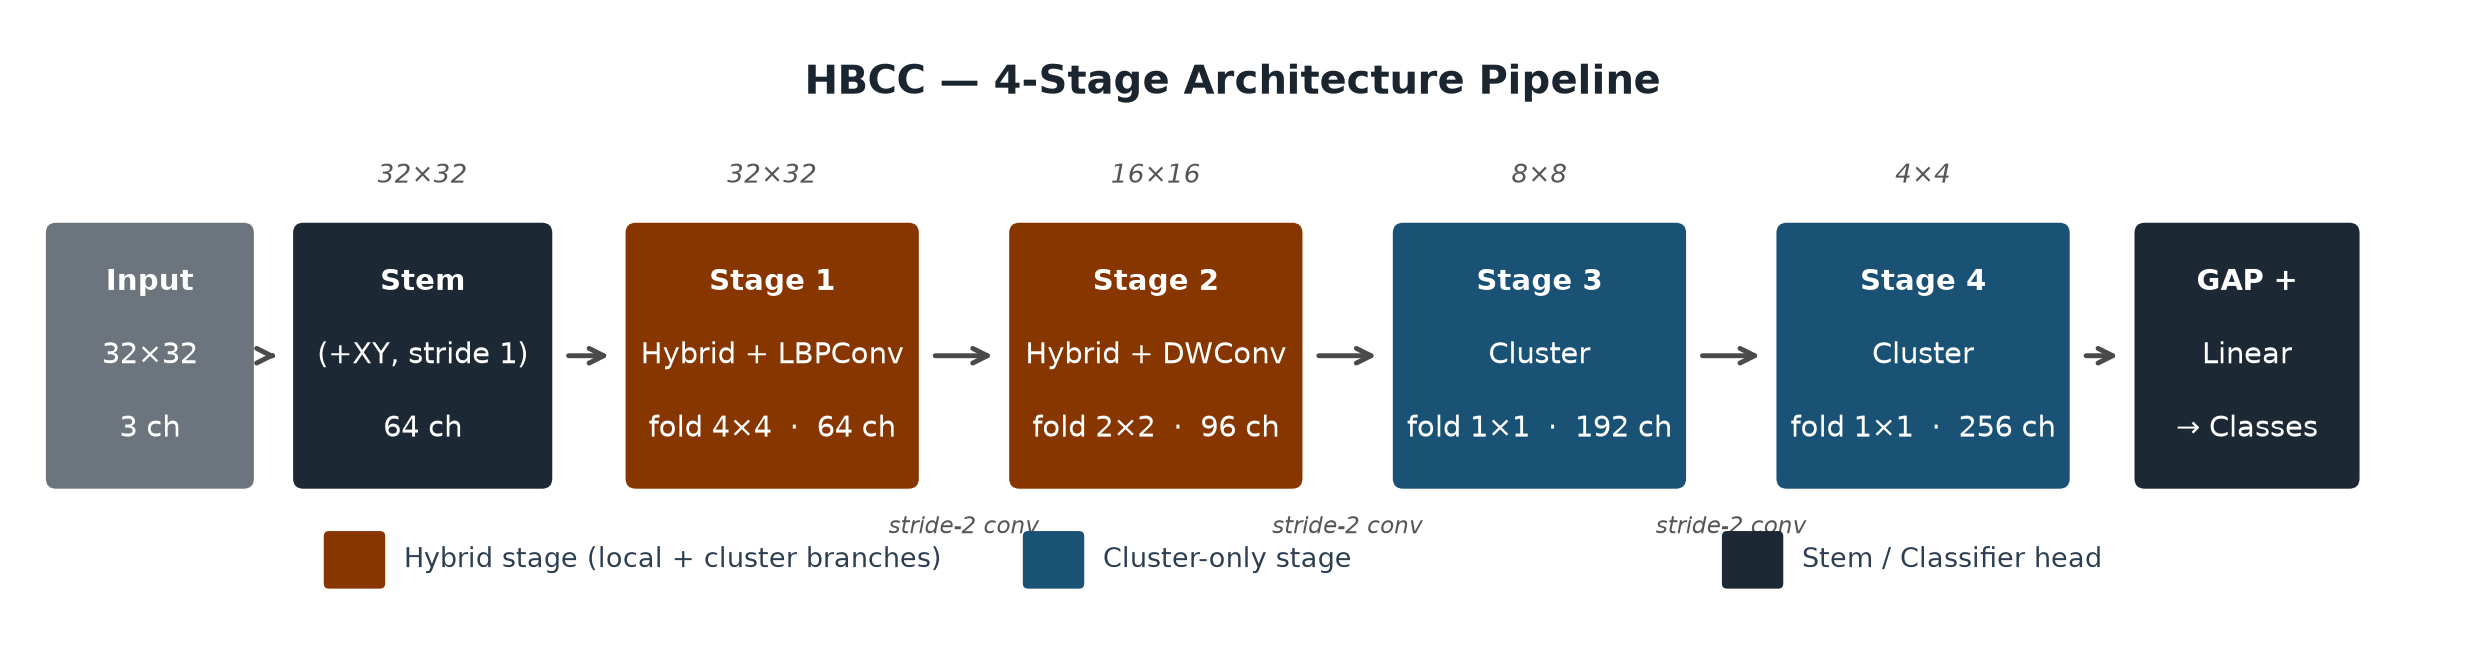
\includegraphics[width=0.97\textwidth]{fig_hbcc_pipeline}
  \caption{Pipeline 4-tầng của HBCC. Màu xanh: Hybrid stage (nhánh
           cục bộ + cluster). Màu đỏ: Cluster-only stage. Độ phân
           giải spatial và số channel $C_i$ ghi chú tại mỗi tầng.}
  \label{fig:pipeline}
\end{figure*}

\subsection{Bổ sung tọa độ $(x,\,y)$}
\label{ssec:coord}

Cosine similarity trên RGB thuần túy không phân biệt hai điểm cùng
màu ở vị trí khác nhau. Chúng tôi bổ sung hai kênh tọa độ chuẩn hóa
về $[0,1]$:
\begin{equation}
  \mathbf{X} = \bigl[\mathbf{I};\;\mathbf{P}_x;\;\mathbf{P}_y\bigr]
  \in\mathbb{R}^{B\times5\times H_0\times W_0},
  \label{eq:coord}
\end{equation}
trong đó $P_x[i,j]=j/(W_0{-}1)$ và $P_y[i,j]=i/(H_0{-}1)$. Bổ
sung tọa độ giúp cluster centers nhận biết vị trí không gian mà
không cần positional encoding tường minh.

\subsection{Cơ chế Context Cluster}
\label{ssec:coc}

Cho feature tensor $\mathbf{X}\in\mathbb{R}^{B\times C\times H\times W}$,
ContextClusterOp thực hiện sáu bước (trên mỗi head độc lập rồi nối
lại):

\noindent\textbf{Bước 1 -- Chiếu đôi:}
\begin{equation}
  \mathbf{F}=\operatorname{Conv}_{1\times1}(\mathbf{X}),\quad
  \mathbf{V}=\operatorname{Conv}_{1\times1}(\mathbf{X}).
  \label{eq:proj}
\end{equation}
$\mathbf{F}$ dùng để so sánh similarity; $\mathbf{V}$ là giá trị cần
aggregate.

\noindent\textbf{Bước 2 -- Đề xuất cluster centers:}
\begin{equation}
  \mathbf{F}_c = \operatorname{AvgPool}_{K_h\times K_w}(\mathbf{F}),\quad
  \mathbf{V}_c = \operatorname{AvgPool}_{K_h\times K_w}(\mathbf{V}).
  \label{eq:centers}
\end{equation}
Với $(K_h,K_w){=}(2,2)$, mỗi tile cho $K{=}4$ cluster centers.
AdaptiveAvgPool không có tham số học và đảm bảo số centers cố định
bất kể kích thước input.

\noindent\textbf{Bước 3 -- Tính similarity và gán cứng:}
\begin{align}
  s_{ij} &= \sigma\!\left(\alpha\cdot
    \frac{\mathbf{f}_{c_i}\cdot\mathbf{f}_j}
         {\|\mathbf{f}_{c_i}\|\|\mathbf{f}_j\|}+\beta\right),
  \label{eq:sim}\\
  m_{ij} &= \mathbf{1}\!\left[i=\operatorname*{arg\,max}_{k}s_{kj}\right],
  \label{eq:mask}
\end{align}
với $\alpha,\beta\in\mathbb{R}$ là tham số học được. Hard assignment
($m_{ij}$) đảm bảo mỗi điểm chỉ đóng góp vào một cluster.

\noindent\textbf{Bước 4 -- Aggregate (trung bình có trọng số):}
\begin{equation}
  \mathbf{g}_i =
  \frac{\mathbf{v}_{c_i}+\displaystyle\sum_j m_{ij}s_{ij}\mathbf{v}_j}
       {1+\displaystyle\sum_j m_{ij}s_{ij}}.
  \label{eq:aggregate}
\end{equation}
Mẫu số $1{+}\sum s_{ij}$ chuẩn hóa bao gồm tự-trọng số của center,
đảm bảo giá trị đầu ra ổn định kể cả khi cluster rỗng.

\noindent\textbf{Bước 5 -- Dispatch:}
\begin{equation}
  \tilde{\mathbf{v}}_j = \sum_i\mathbf{g}_i\cdot m_{ij}\cdot s_{ij}.
  \label{eq:dispatch}
\end{equation}
Thông tin tổng hợp được phân phối ngược về mỗi điểm theo trọng số.

\noindent\textbf{Bước 6 -- Chiếu đầu ra:}
$\mathbf{Y}=\operatorname{Conv}_{1\times1}(\tilde{\mathbf{V}})$.

\subsection{Fold partitioning}

Ở resolution cao ($32\!\times\!32$, $16\!\times\!16$), phân cụm toàn
cục tạo cluster quá lớn, làm mờ chi tiết cục bộ (global
over-smoothing). Chúng tôi chia feature map thành
$F_h\!\times\!F_w$ tile không chồng lấp:
\begin{equation}
  (B,\,C,\,F_h h,\,F_w w)\;\longrightarrow\;(B F_h F_w,\,C,\,h,\,w).
  \label{eq:fold}
\end{equation}
CoC áp dụng độc lập trong từng tile rồi reshape ngược lại. Fold thu
nhỏ theo tầng: $4\!\times\!4$ (Tầng~1, $32\!\times\!32$),
$2\!\times\!2$ (Tầng~2, $16\!\times\!16$), $1\!\times\!1$
(Tầng~3--4, toàn cục).

\subsection{Hybrid Cluster Block}
\label{ssec:hybrid}

Hình~\ref{fig:hybrid} mô tả cấu trúc. Với local ratio $\rho\in[0,1]$:
nhánh cục bộ có $C_l{=}\lfloor C\rho\rceil$ channel; nhánh cluster
có $C_c{=}C-C_l$ channel.

\noindent\textbf{Token mixing:}
\begin{align}
  [\mathbf{x}_c;\,\mathbf{x}_l] &=
    \operatorname{split}\!\bigl(\operatorname{BN}(\mathbf{x}),[C_c,C_l]\bigr),
  \label{eq:split}\\
  \mathbf{y} &= \operatorname{Fuse}_{1\times1}\!\Bigl(
    \operatorname{Shuffle}\bigl[\operatorname{CoC}(\mathbf{x}_c);\;
    \operatorname{Local}(\mathbf{x}_l)\bigr]\Bigr),
  \label{eq:mix}\\
  \mathbf{x} &\leftarrow \mathbf{x}+
    \operatorname{DropPath}(\bm{\gamma}_1\odot\mathbf{y}).
  \label{eq:skip1}
\end{align}

\noindent\textbf{MLP:}
\begin{equation}
  \mathbf{x}\leftarrow\mathbf{x}+
  \operatorname{DropPath}\!\bigl(
    \bm{\gamma}_2\odot\operatorname{MLP}(\operatorname{BN}(\mathbf{x}))\bigr),
  \label{eq:skip2}
\end{equation}
trong đó $\bm{\gamma}_1,\bm{\gamma}_2\in\mathbb{R}^C$ là layer-scale
khởi tạo tại $10^{-5}$. Channel Shuffle~\cite{Ma2018ShuffleNetV2}
trao đổi thông tin giữa hai nhánh trước khi fuse bằng $1\!\times\!1$
convolution. Khi $\rho{=}0$ (Tầng~3--4), nhánh cục bộ, Shuffle, và
Fuse đều bị bỏ qua.

\begin{figure}[!t]
  \centering
  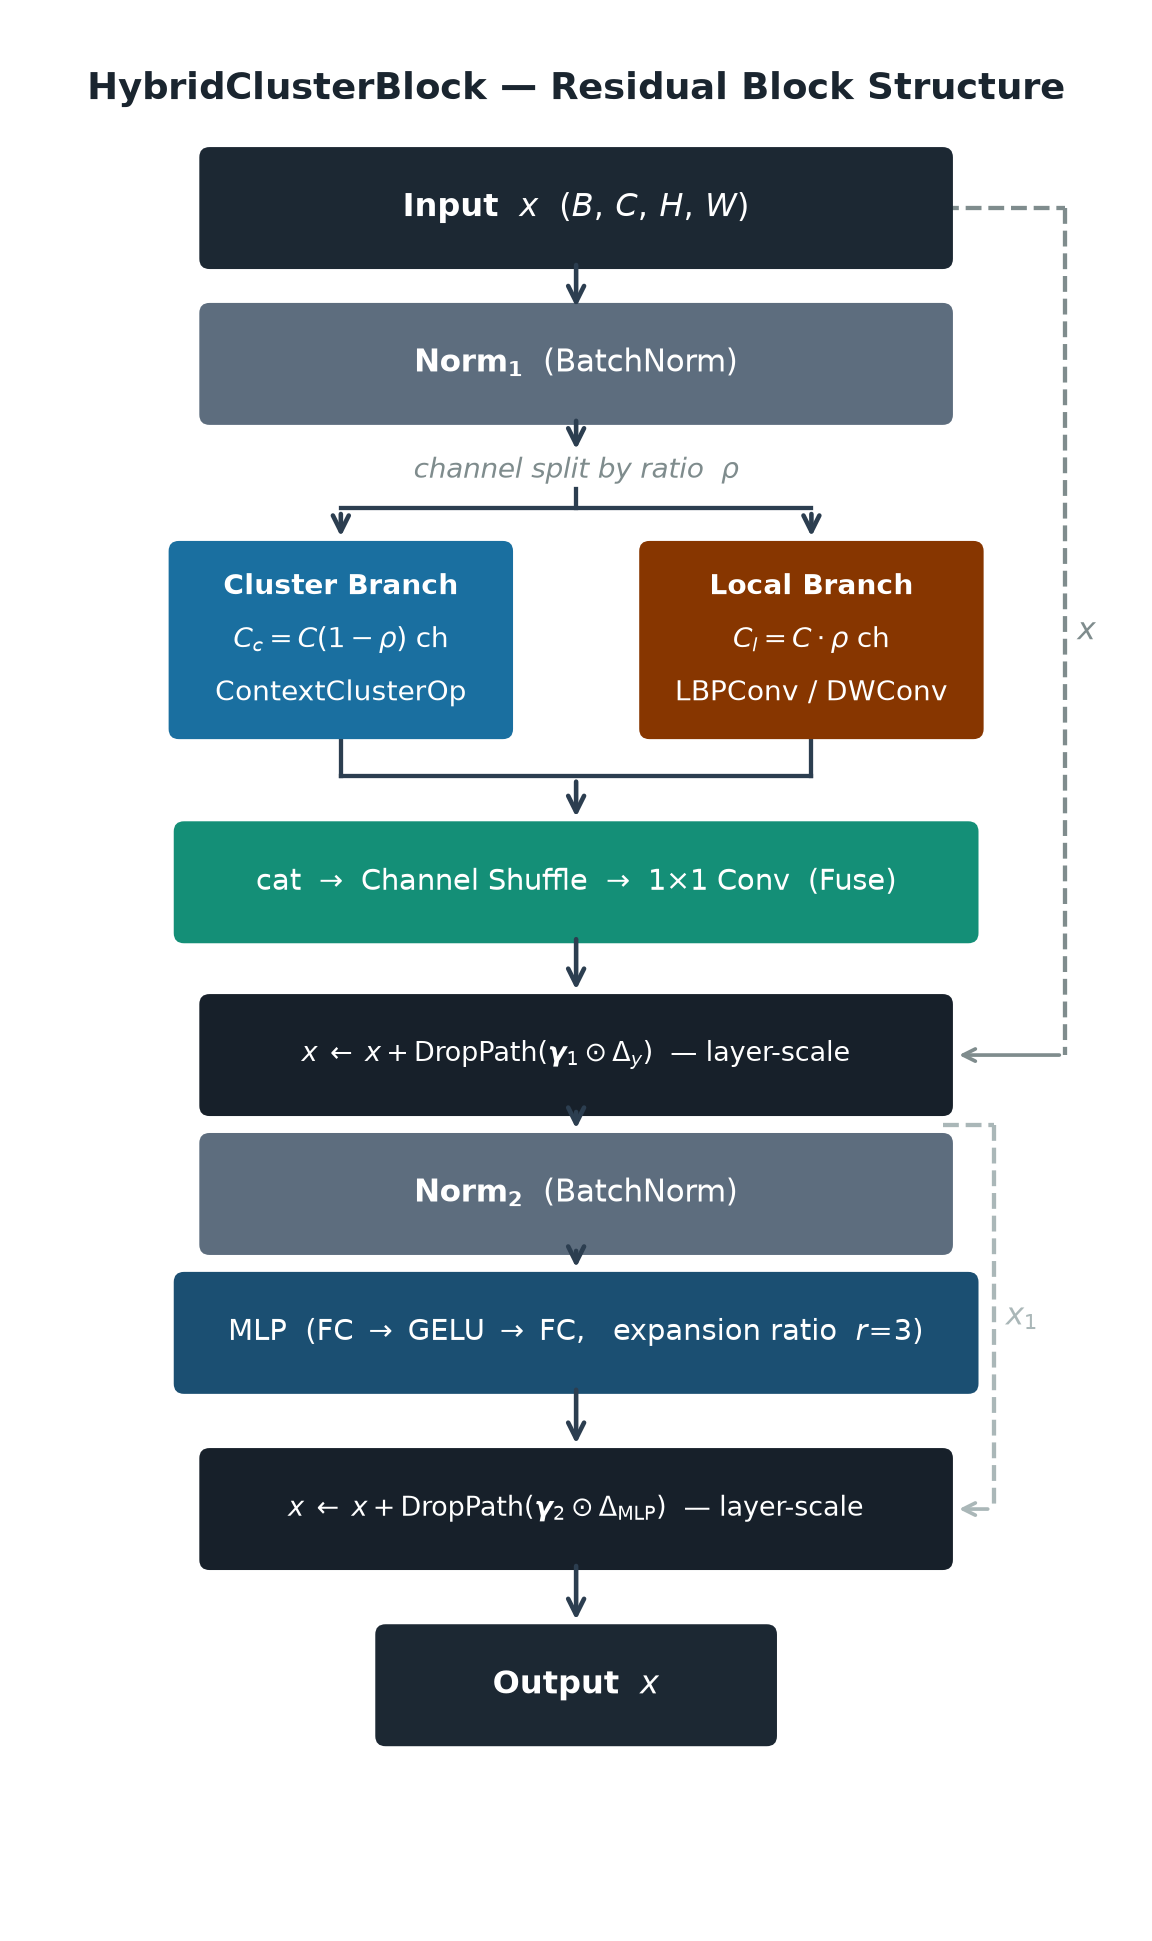
\includegraphics[width=0.95\columnwidth]{fig_hybrid_block}
  \caption{Cấu trúc Hybrid Cluster Block. Nhánh xanh: CoC
           ($C_c{=}C(1{-}\rho)$ channel). Nhánh cam: Local branch
           ($C_l{=}C\rho$ channel). Fuse qua channel shuffle và
           $1\!\times\!1$ conv. Layer-scale $\bm{\gamma}$ khởi
           tạo $10^{-5}$.}
  \label{fig:hybrid}
\end{figure}

\subsection{Nhánh cục bộ}

\noindent\textbf{LBPConv (Tầng~1, $32\!\times\!32$).}
Áp dụng công thức~\eqref{eq:lbp} trên từng channel, tạo binary
descriptor rotation-invariant. Chi phí chỉ là phép trừ và ngưỡng
nhị phân -- gần như không tốn MACs. Phù hợp với Tầng~1 nơi kết cấu
vi mô (đường nét, cạnh) còn phong phú và quan trọng hơn ngữ cảnh
toàn cục.

\noindent\textbf{DWConv (Tầng~2, $16\!\times\!16$).}
Depthwise convolution $3\!\times\!3$ xử lý từng channel độc lập với
chi phí $1/C$ so với standard convolution. Ở Tầng~2, kết cấu cục bộ
đã được xử lý một phần ở Tầng~1; DWConv cung cấp receptive field
không gian bổ sung với chi phí tối thiểu.

\noindent\textbf{Pure Cluster (Tầng~3--4, $8\!\times\!8$,
$4\!\times\!4$).}
Ở resolution thấp, kết cấu cục bộ không còn ý nghĩa và phân cụm
toàn cục khai thác quan hệ toàn cảnh hiệu quả ($\rho{=}0$).

\subsection{Phân tích suy biến token và lựa chọn stem\_stride}
\label{sec:degeneracy}

Số điểm trên mỗi cụm trong một vùng fold là:
\begin{equation}
  r = \frac{(H/F_h)\cdot(W/F_w)}{K_h\cdot K_w}.
  \label{eq:ratio}
\end{equation}
Để phân cụm có ý nghĩa, $r\geq4$ là cần thiết. Với
\textbf{stem\_stride=2} trên ảnh $32\!\times\!32$:
\begin{itemize}
  \item Tầng~4: $2\!\times\!2=4$ điểm, proposals$(2,2)$ tạo 4 tâm
        $\Rightarrow r=1$ -- mỗi cụm chứa đúng \emph{một điểm}, toán
        tử phân cụm là hằng đồng nhất, không học được.
  \item Tầng~3: $4\!\times\!4=16$ điểm, fold$(1,1)$,
        proposals$(2,2)$ $\Rightarrow r=4$ -- chỉ đủ ngưỡng tối thiểu.
\end{itemize}

Giải pháp: giảm \textbf{stem\_stride xuống 1}, khiến sau stem còn
$32\!\times\!32=1024$ điểm. Kết hợp với fold theo từng tầng, $r=16$
đạt được nhất quán trên toàn pipeline:
\begin{itemize}
  \item Tầng~1: fold$(4,4)$ trên $32\!\times\!32$:
        $8\!\times\!8=64$ điểm/vùng, 4 tâm $\Rightarrow r=16$. \checkmark
  \item Tầng~2: fold$(2,2)$ trên $16\!\times\!16$:
        $8\!\times\!8=64$ điểm/vùng, 4 tâm $\Rightarrow r=16$. \checkmark
  \item Tầng~3: fold$(1,1)$ trên $8\!\times\!8$:
        64 điểm, 4 tâm $\Rightarrow r=16$. \checkmark
  \item Tầng~4: fold$(1,1)$, proposals$(1,1)$ trên $4\!\times\!4$:
        16 điểm, 1 tâm $\Rightarrow r=16$. \checkmark
\end{itemize}

Để bù lại chi phí tính toán tăng (diện tích feature map gấp $4\times$
ở mỗi tầng), số khối mỗi tầng được thu hẹp từ $[2,2,4,2]$ xuống
$[1,1,2,1]$. Cấu hình cuối (Bảng~\ref{tab:stages}) giữ tổng chi phí
ở mức hợp lý trong khi đảm bảo toán tử phân cụm hoạt động đúng trên
toàn bộ các tầng.

\subsection{Cấu hình tầng}

Bảng~\ref{tab:stages} liệt kê cấu hình chi tiết. MLP expansion ratio:
3,0. Proposal size $(K_h,K_w){=}(2,2)$ cho tất cả tầng (4 cluster
centers mỗi tile), ngoại trừ Tầng~4 dùng $(1,1)$ để global context.

\begin{table}[!t]
  \caption{Cấu hình tầng của HBCC-Small (S) và HBCC-Medium (M).
           $d$: số block; $C$: embed dim; $\rho$: local ratio.}
  \label{tab:stages}
  \centering
  \renewcommand{\arraystretch}{1.15}
  \resizebox{\linewidth}{!}{%
  \begin{tabular}{c c c c c c c c}
    \toprule
    Tầng & Res. & Chế độ & Cục bộ & $\rho$ & Fold &
      $d_{S/M}$ & $C_{S}/C_{M}$ \\
    \midrule
    1 & $32^2$ & Hybrid  & LBPConv & 0,5 & $4\times4$ & 1/1 & 48/64   \\
    2 & $16^2$ & Hybrid  & DWConv  & 0,5 & $2\times2$ & 1/1 & 80/96   \\
    3 & $8^2$  & Cluster & ---     & 0,0 & $1\times1$ & 2/2 & 160/192 \\
    4 & $4^2$  & Cluster & ---     & 0,0 & $1\times1$ & 1/1 & 224/256 \\
    \bottomrule
  \end{tabular}}
\end{table}

% ============================================================
\section{Thiết Lập Thực Nghiệm}
\label{sec:exp}

\subsection{Bộ dữ liệu và phân chia dữ liệu}

Chúng tôi đánh giá trên CIFAR-10 (10 lớp, 60.000 ảnh $32\!\times\!32$)
và CIFAR-100 (100 lớp, 60.000 ảnh)~\cite{Krizhevsky2009Cifar}. Phân
chia dữ liệu cố định đồng nhất cho tất cả mô hình: 45.000 train /
5.000 validation / 10.000 test, random seed~42, đảm bảo tính công
bằng trong so sánh. Tập xác thực dùng để chọn điểm kiểm tra tốt nhất
(\texttt{best.pth}); tập test chính thức 10.000 ảnh chỉ được dùng
một lần để báo cáo kết quả cuối cùng.

\subsection{Công thức huấn luyện}

\begin{table}[!t]
  \caption{Training recipe của HBCC-Small và HBCC-Medium.}
  \label{tab:train}
  \centering
  \renewcommand{\arraystretch}{1.15}
  \resizebox{\linewidth}{!}{%
  \begin{tabular}{l l}
    \toprule
    Siêu tham số & Giá trị \\
    \midrule
    Optimizer               & AdamW \\
    Learning rate           & $1\times10^{-3}$ \\
    Weight decay            & 0,05 \\
    LR schedule             & Cosine annealing \\
    Warmup epochs           & 5 \\
    Total epochs (CE)       & 300 \\
    Total epochs (KD)       & 250 \\
    Label smoothing         & 0,1 \\
    RandAugment~\cite{Cubuk2020RandAugment} & $N{=}2,\ M{=}9$ \\
    MixUp~\cite{Zhang2018Mixup} $\alpha$    & 0,2 \\
    CutMix~\cite{Yun2019CutMix} $\alpha$, $p$ & 1,0;\ 0,5 \\
    Random Erasing $p$      & 0,25 \\
    AMP (mixed precision)   & Có \\
    Drop path (Small/Med.)  & 0,05 / 0,08 \\
    \bottomrule
  \end{tabular}}
\end{table}

HBCC-Small và HBCC-Medium được huấn luyện với recipe mạnh
(Bảng~\ref{tab:train}). Các mô hình đối chứng (ResNet-18,
MobileNetV2, ShuffleNetV2, CoC-baseline) được huấn luyện 300 epoch
với tăng cường dữ liệu chuẩn (random crop + lật ngang + chuẩn hóa).
Bất đối xứng recipe là hạn chế được thừa nhận (Phần~\ref{sec:limitations}).

\subsection{Chưng cất tri thức}
\label{ssec:kd_setup}

Để tăng thêm độ chính xác mà không tăng số tham số tại thời điểm
suy luận, chúng tôi áp dụng response-based KD~\cite{Hinton2015Distillation}
với giáo viên ResNet-18 được huấn luyện từ đầu trên cùng tập dữ liệu
(đạt 96,48\% trên CIFAR-10 và 79,57\% trên CIFAR-100). Hàm mất mát:
\begin{equation}
  \mathcal{L}_{\mathrm{KD}} = (1-\alpha)\,\mathcal{L}_{\mathrm{CE}}(p,y)
  + \alpha T^2\,\mathrm{KL}\!\left(
    \sigma\!\left(\tfrac{z_s}{T}\right)\Big\|
    \sigma\!\left(\tfrac{z_t}{T}\right)\right),
  \label{eq:kd}
\end{equation}
trong đó $z_s, z_t$ là logit học sinh/giáo viên, $y$ là nhãn cứng,
$\alpha{=}0{,}5$ và $T{=}4{,}0$. Giáo viên được giữ cố định trong
suốt quá trình huấn luyện KD. Số epoch giảm từ 300 xuống 250 do
mỗi epoch KD tốn thêm lượt truyền xuôi qua giáo viên.

\subsection{Đo lường hiệu năng}

\textbf{Tham số và MACs} đo bằng \texttt{fvcore} trước khi huấn
luyện. Lưu ý: \texttt{fvcore} không đếm \texttt{scatter\_},
\texttt{sigmoid}, \texttt{sum} trong clustering ops; MACs báo cáo
cho HBCC là \emph{giới hạn dưới}.

\textbf{Độ trễ} đo trên GPU Tesla~T4 (PyTorch~2.x, CUDA~12.x),
batch size~1, 30 lần warmup và 100 lần đo, chế độ latency\_strict
(đồng bộ hóa CUDA sau mỗi lần lặp) -- phản ánh single-sample
latency cho suy luận thời gian thực.

\textbf{Bộ nhớ đỉnh} ghi lại bằng lệnh \texttt{max\_memory\_\allowbreak allocated}
của \texttt{torch.cuda}. \textbf{Hồ sơ toán tử} thu thập qua
\texttt{torch.profiler\allowbreak.profile} với
\texttt{activities=[CUDA]}.

\subsection{Mô hình đối chứng}

\begin{itemize}
  \item \textbf{ResNet-18}~\cite{He2016ResNet}: thay conv
        $7\!\times\!7$ stride-2 bằng conv $3\!\times\!3$ stride-1,
        bỏ max-pool đầu. Cũng đóng vai giáo viên KD.
  \item \textbf{MobileNetV2}~\cite{Sandler2018MobileNetV2}: stem
        conv $3\!\times\!3$ stride-1, bỏ max-pool.
  \item \textbf{ShuffleNetV2-x1.0}~\cite{Ma2018ShuffleNetV2}:
        chỉnh tương tự, stride đầu giảm xuống 1.
  \item \textbf{CoC-baseline}: CoC phân cụm toàn cục ($\rho{=}0$)
        ở mọi tầng, không có nhánh cục bộ -- đối chứng kiến trúc
        trực tiếp để cô lập đóng góp của nhánh cục bộ.
\end{itemize}

% ============================================================
\section{Kết Quả và Thảo Luận}
\label{sec:results}

\subsection{Kết quả trên CIFAR-10}

Bảng~\ref{tab:cifar10} so sánh tám mô hình trên CIFAR-10.
HBCC-Medium+KD đạt \textbf{95,36\%} -- cao nhất trong nhóm mô hình
nhẹ, chỉ thấp hơn ResNet-18 ($-$1,12\%) trong khi sử dụng
\textbf{6,34×} ít tham số (1,76M so với 11,17M) và
\textbf{4,01×} ít MACs (138,8M so với 556,7M). Các so sánh nổi bật:

\begin{itemize}
  \item HBCC-Small+KD (1,27M) so với ShuffleNetV2 (1,26M):
        $+$3,25\% top-1 ở cùng ngân sách tham số.
  \item HBCC-Small+KD (1,27M) so với MobileNetV2 (2,24M):
        $+$3,89\% top-1 với ít tham số hơn đáng kể.
  \item HBCC-Medium+KD (1,76M) so với CoC-baseline (2,40M):
        $+$7,02\% top-1, ít tham số hơn \emph{và nhanh hơn} (8,09ms
        so với 11,71ms). HBCC vừa chính xác hơn vừa nhanh hơn CoC,
        xác nhận lợi ích kép của nhánh cục bộ: giảm độ trễ ở tầng
        phân giải cao và giữ lại thông tin biên/kết cấu.
\end{itemize}

\begin{table}[!t]
  \caption{So sánh trên CIFAR-10. \textbf{In đậm}: tốt nhất trong
           nhóm nhẹ. \texttt{+KD}: huấn luyện với chưng cất tri thức.}
  \label{tab:cifar10}
  \centering
  \renewcommand{\arraystretch}{1.15}
  \resizebox{\linewidth}{!}{%
  \begin{tabular}{l c r r r r}
    \toprule
    Mô hình & Top-1(\%) & Params(M) & MACs(M) & Trễ(ms) & Mem(MB) \\
    \midrule
    ResNet-18             & 96,48 & 11,17 & 556,66 &  3,03 & 326,4 \\
    \midrule
    HBCC-Medium+KD        & \textbf{95,36} & 1,76 & 138,81 & 8,09 & 481,4 \\
    HBCC-Small+KD         & 94,93 &  1,27 &  92,34 &  8,41 & 363,6 \\
    HBCC-Medium (CE)      & 94,45 &  1,76 & 138,81 &  7,87 & 481,4 \\
    HBCC-Small (CE)       & 94,00 &  1,27 &  92,34 &  7,82 & 363,6 \\
    ShuffleNetV2-x1.0     & 91,68 &  1,26 &  46,13 &  6,26 &  94,8 \\
    MobileNetV2           & 91,04 &  2,24 &  25,57 &  4,76 & 123,4 \\
    CoC-baseline          & 88,34 &  2,40 &  34,37 & 11,71 & \textbf{71,8} \\
    \bottomrule
  \end{tabular}}
\end{table}

\subsection{Kết quả trên CIFAR-100}

Bảng~\ref{tab:cifar100} cho thấy HBCC-Medium+KD đạt \textbf{77,68\%}
top-1 -- cao nhất trong tất cả mô hình nhẹ và chỉ kém ResNet-18
($-$1,89\%). HBCC-Small+KD (1,27M) vượt ShuffleNetV2 (1,36M)
$+$0,29\% ở cùng phân khúc tham số. Quan trọng: nếu không có KD,
HBCC-Medium (75,59\%) và HBCC-Small (75,40\%) đều \emph{thấp hơn}
ShuffleNetV2 (76,46\%) -- KD là yếu tố quyết định giúp HBCC vượt
qua ShuffleNetV2 trên CIFAR-100.

\begin{table}[!t]
  \caption{So sánh trên CIFAR-100. \textbf{In đậm}: tốt nhất trong
           nhóm nhẹ. \texttt{+KD}: huấn luyện với chưng cất tri thức.}
  \label{tab:cifar100}
  \centering
  \renewcommand{\arraystretch}{1.15}
  \resizebox{\linewidth}{!}{%
  \begin{tabular}{l c c r r r}
    \toprule
    Mô hình & Top-1(\%) & Top-5(\%) & Params(M) & MACs(M) & Trễ(ms) \\
    \midrule
    ResNet-18             & 79,57 & 93,97 & 11,22 & 556,71 &  3,03 \\
    \midrule
    HBCC-Medium+KD        & \textbf{77,68} & 93,86 & 1,78 & 138,83 & 7,83 \\
    HBCC-Small+KD         & 76,75 & \textbf{93,95} & 1,30 &  92,36 & 7,51 \\
    ShuffleNetV2-x1.0     & 76,46 & 93,43 &  1,36 &  46,22 &  5,77 \\
    HBCC-Medium (CE)      & 75,59 & 92,76 &  1,78 & 138,83 &  7,69 \\
    HBCC-Small (CE)       & 75,40 & 92,93 &  1,30 &  92,36 &  7,59 \\
    MobileNetV2           & 73,75 & 92,54 &  2,35 &  25,67 &  4,77 \\
    CoC-baseline          & 72,01 & 90,70 &  2,42 &  34,40 & 11,21 \\
    \bottomrule
  \end{tabular}}
\end{table}

\subsection{Hiệu quả của chưng cất tri thức}

Bảng~\ref{tab:kd_gain} so sánh mức tăng do KD. Hiệu quả KD lớn hơn
rõ rệt trên CIFAR-100: $+$2,09\%/$+$1,35\% cho Medium/Small, gần
gấp đôi so với CIFAR-10 ($+$0,91\%/$+$0,93\%). Điều này phù hợp
lý thuyết: trên 100 lớp mịn, phân phối mềm của giáo viên mang nhiều
thông tin liên lớp hơn (ví dụ: xe máy và xe hơi chia sẻ cấu trúc
bánh xe), trong khi trên CIFAR-10 (10 lớp tương đối tách biệt)
thông tin đó ít phong phú hơn.

\begin{table}[!t]
  \caption{Mức tăng top-1 do KD ($\Delta$ = KD $-$ CE).}
  \label{tab:kd_gain}
  \centering
  \renewcommand{\arraystretch}{1.15}
  \begin{tabular}{lcc}
    \toprule
    Mô hình & $\Delta$ CIFAR-10 (\%) & $\Delta$ CIFAR-100 (\%) \\
    \midrule
    HBCC-Medium & $+$0,91 & $+$2,09 \\
    HBCC-Small  & $+$0,93 & $+$1,35 \\
    \bottomrule
  \end{tabular}
\end{table}

\subsection{Phân tích Pareto}

Hình~\ref{fig:pareto10} và~\ref{fig:pareto100} biểu diễn accuracy
vs.\ số tham số và accuracy vs.\ latency. Cả HBCC-Small+KD và
HBCC-Medium+KD đều nằm ở vùng Pareto-dominant trên trục tham số:
accuracy cao hơn với tham số ít hơn so với mọi baseline nhẹ. Trên
trục latency, HBCC có latency cao hơn (phân tích ở
Mục~\ref{ssec:latency}) nhưng accuracy cũng cao hơn rõ ràng so với
MobileNetV2 và ShuffleNetV2. HBCC không Pareto-dominant so với
ResNet-18 trên trục latency, nhưng hoàn toàn Pareto-dominant trên
trục tham số và vượt trội về accuracy/params so với các mô hình nhẹ
khác.

\begin{figure}[!t]
  \centering
  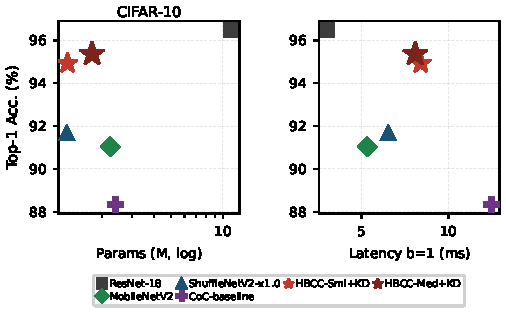
\includegraphics[width=\columnwidth]{pareto_cifar10}
  \caption{Pareto frontier trên CIFAR-10. Trái: accuracy vs.\ số
           tham số (log scale). Phải: accuracy vs.\ latency lô~1 (ms).
           Sao~($\bigstar$): HBCC+KD; vòng tròn rỗng: HBCC~CE;
           mũi tên: mức tăng do KD. HBCC+KD nằm ở vùng trên-trái
           so với các mô hình nhẹ cùng phân khúc tham số.}
  \label{fig:pareto10}
\end{figure}

\begin{figure}[!t]
  \centering
  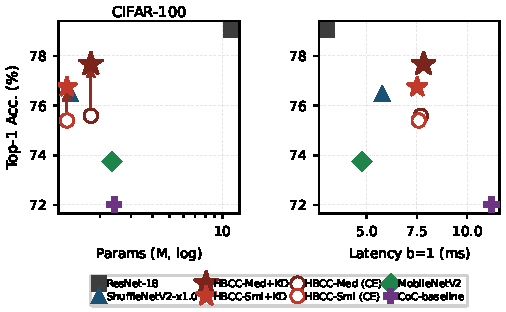
\includegraphics[width=\columnwidth]{pareto_cifar100}
  \caption{Pareto frontier trên CIFAR-100. Mũi tên trong panel trái
           thể hiện mức tăng accuracy nhờ KD (+2,09\% cho Medium,
           +1,35\% cho Small). HBCC-Sml+KD và HBCC-Med+KD đều vượt
           ShuffleNetV2 ở cùng phân khúc tham số.}
  \label{fig:pareto100}
\end{figure}

\subsection{Phân tích latency: vì sao ít MACs hơn vẫn chậm hơn}
\label{ssec:latency}

Mặc dù HBCC-Medium dùng ít MACs hơn ResNet-18, latency batch-1 của
HBCC-Medium lại cao hơn ($\approx\!8$~ms vs $\approx\!3$~ms). Nguyên
nhân là \textit{operator fragmentation} được xác nhận qua CUDA
profiling:

\noindent\textbf{ResNet-18} dành $\approx\!94\%$ thời gian CUDA trong
một kernel duy nhất (\texttt{aten::cudnn\_convolution}) -- được cuDNN
tối ưu hóa kỹ qua Winograd, FFT-based convolution và implicit GEMM,
tận dụng tối đa tensor core của GPU.

\noindent\textbf{HBCC-Medium} phân tán thời gian trên nhiều kernel
nhỏ: tích chập $1\!\times\!1$ (\texttt{conv2d}, $\approx\!25\%$),
nhân ma trận (\texttt{mm/bmm}, $\approx\!20\%$), chuẩn hóa vector
(\texttt{linalg\_vector\_norm}, $\approx\!10\%$), các phép tổng hợp
cụm (\texttt{mul/sum}, $\approx\!15\%$), và đề xuất tâm cụm
(\texttt{adaptive\_avg\_pool2d}, $\approx\!10\%$). Mỗi lần khởi chạy
kernel tốn chi phí cố định (kernel launch overhead), và nhiều kernel
nhỏ nối tiếp không khai thác song song hóa GPU tốt bằng một kernel
tích chập lớn.

Đây là sự khác biệt giữa \textit{số phép toán số học} (MACs) và
\textit{chi phí scheduling kernel} (latency wall-clock), nhất quán
với nguyên tắc ShuffleNetV2: MACs không phải chỉ số đáng tin cậy
để dự đoán tốc độ thực đo. HBCC vẫn nhanh hơn CoC thuần
$30\!-\!35\%$ (8ms vs 11ms), cho thấy thiết kế lai đã cải thiện
đáng kể so với phân cụm toàn cục.

\subsection{Trả lời câu hỏi nghiên cứu}

\noindent\textbf{(CQ1) -- Kiến trúc lai có cải thiện đồng thời
accuracy và hiệu quả?}

Kết quả trả lời khẳng định trên cả hai phương diện:
\begin{itemize}
  \item \textit{Accuracy:} HBCC-Medium+KD vượt tất cả baseline nhẹ
        -- ShuffleNetV2 ($+$3,68\% CIFAR-10, $+$1,22\% CIFAR-100),
        MobileNetV2 ($+$4,32\% CIFAR-10, $+$3,93\% CIFAR-100), và
        CoC-baseline ($+$7,02\% CIFAR-10, $+$5,67\% CIFAR-100).
  \item \textit{Hiệu quả:} HBCC-Small+KD đạt 94,93\% trên CIFAR-10
        với chỉ 1,27M tham số và 92,3M MACs -- Pareto-dominant so
        với ShuffleNetV2 (1,26M, 91,68\%) và MobileNetV2 (2,24M,
        91,04\%).
\end{itemize}
Kết quả nhất quán với giả thuyết rằng kết hợp cục bộ (tần số cao)
và phân cụm (quan hệ vùng) bổ sung cho nhau, tạo ra mô hình tổng
thể tốt hơn cả hai thành phần đơn lẻ.

\noindent\textbf{(CQ2) -- Chiến lược phân bổ tầng nào là tối ưu?}

Khoảng cách lớn giữa HBCC-Medium+KD và CoC-baseline
(6,11--7,02 điểm CIFAR-10, 5,67 điểm CIFAR-100) cung cấp bằng chứng
mạnh rằng \emph{hybrid ở Tầng~1--2, pure cluster ở Tầng~3--4} là
chiến lược hiệu quả. Lý giải theo tần số không gian: ở
$32\!\times\!32$ và $16\!\times\!16$, ảnh còn chứa nhiều thông tin tần
số cao (kết cấu, cạnh) mà convolution cục bộ nắm bắt tốt hơn phân
cụm; ở $8\!\times\!8$ và $4\!\times\!4$, thông tin đã đủ trừu tượng
hóa để phân cụm toàn cục hoạt động hiệu quả. Fold partitioning thu
nhỏ dần phản ánh nguyên tắc này.

% ============================================================
\section{Hạn Chế}
\label{sec:limitations}

\textbf{Một lần chạy duy nhất.} Mỗi mô hình được train một lần với
seed cố định; kết quả là point estimate không có confidence interval.
Khoảng cách 0,29\% giữa HBCC-Small+KD và ShuffleNetV2 trên CIFAR-100
cần được xác nhận qua ít nhất 5 seed với t-test hoặc bootstrap trước
khi khẳng định có ý nghĩa thống kê.

\textbf{Bất đối xứng training recipe.} HBCC được train 300 epoch với
RandAugment, MixUp, CutMix và RandomErasing, trong khi baseline chỉ
dùng augmentation cơ bản. Một phần accuracy advantage có thể đến từ
recipe mạnh hơn. Ablation với cùng recipe cho tất cả mô hình là cần
thiết để tách bạch đóng góp kiến trúc thuần túy.

\textbf{MACs là lower bound.} \texttt{fvcore} không đếm các phép
\texttt{scatter}, sigmoid, và sum trong clustering ops; chi phí tính
toán thực tế của HBCC cao hơn số báo cáo.

\textbf{Chỉ đánh giá trên CIFAR-10/100.} Ảnh $32\!\times\!32$ là
điều kiện thuận lợi cho phân tích suy biến token và lựa chọn fold.
Kết quả có thể không tổng quát trực tiếp sang ImageNet
($224\!\times\!224$); cấu hình fold và proposals cần điều chỉnh lại.

\textbf{Độ trễ vẫn cao hơn các mô hình tích chập nhẹ.} HBCC chậm
hơn ShuffleNetV2 $\approx\!1,3\!\times$ và chậm hơn ResNet-18
$\approx\!2,6\!\times$. Hướng giải quyết: operator fusion qua
\texttt{torch.compile}, hoặc kernel XNOR/popcount tùy chỉnh (Track~B).

\textbf{Track B chưa hoàn thành.} Cosine similarity sẽ được thay
bằng Hamming distance (XOR + popcount) để tận dụng phần cứng nhị
phân~\cite{Courbariaux2016BNN,Bengio2013STE}. Hiện tại BOPs được
tính lý thuyết; XNOR kernel thực trên ARM/FPGA chưa được implement.

% ============================================================
\section{Kết Luận và Đề Nghị}
\label{sec:conclusion}

Bài báo đề xuất HBCC, kiến trúc lai kết hợp Context Cluster với xử
lý cục bộ (LBPConv, DWConv) theo nguyên tắc lũy tiến: hybrid stages
ở resolution cao; pure cluster stages ở resolution thấp. Fold
partitioning, coordinate injection, channel shuffle và layer-scale là
các cơ chế hỗ trợ. Khắc phục suy biến token qua stem\_stride=1 và
thu hẹp số khối là đóng góp kỹ thuật cốt lõi đảm bảo toán tử phân
cụm hoạt động đúng trên toàn pipeline. KD từ ResNet-18 tăng thêm
độ chính xác mà không tăng tham số thời suy luận.

\noindent\textbf{(CQ1)} HBCC-Medium+KD Pareto-dominant trên trục tham
số, khẳng định kiến trúc lai cải thiện đồng thời accuracy và hiệu
quả. \textbf{(CQ2)} Khoảng cách $>$6 điểm so với CoC-baseline xác
nhận chiến lược hybrid tại Tầng~1--2 và pure cluster tại Tầng~3--4
là tối ưu, nhất quán với lý thuyết tần số không gian.

\noindent\textbf{Đề xuất 1 --- Ứng dụng edge AI:}
HBCC-Small+KD (1,27M tham số, 92,3M MACs) phù hợp cho thiết bị
nhúng phân loại ảnh $32$--$64$ pixel -- ví dụ camera kiểm tra chất
lượng sản phẩm, hệ thống phân loại nhãn dán trên vi điều khiển ARM
Cortex-M với bộ nhớ dưới 2~MB.

\noindent\textbf{Đề xuất 2 --- HBCC-BitEdge (Track B):}
Triển khai Hamming distance (XOR + popcount) thay cosine similarity
và phát triển XNOR kernel tối ưu trên phần cứng, nhằm giảm latency
về mức cạnh tranh với các mô hình tích chập trong khi duy trì
accuracy advantage trên tham số.

\noindent\textbf{Đề xuất 3 --- Chuẩn hóa thực nghiệm:}
(a)~Train tất cả baseline với cùng recipe để tách bạch đóng góp kiến
trúc; (b)~lặp lại ít nhất 5 seed và báo cáo trung bình $\pm$ độ
lệch chuẩn; (c)~đánh giá HBCC trên ImageNet-1k với fold size điều
chỉnh để kiểm tra khả năng mở rộng quy mô.

% ============================================================
\section*{Lời Cảm Ơn}

Nhóm tác giả xin cảm ơn PGS.TS. Lê Hoàng Thái đã định hướng và góp
ý trong suốt quá trình nghiên cứu. Toàn bộ thực nghiệm được thực
hiện trên hạ tầng GPU miễn phí của Kaggle (Tesla~T4).

% ============================================================
\clearpage
\bibliographystyle{IEEEtran}
\bibliography{references}

\end{document}
